\documentclass{beamer}

% Beamer style
\usetheme[style=plain]{uu}


%% Standard packages
\usepackage{graphicx}
\usepackage{mathtools}
\usepackage{amssymb}
\usepackage{amsfonts}
\usepackage{hyperref}
\usepackage{color}

%% unicode support, for text and code :)
\usepackage{ucs}
\usepackage{autofe}
\usepackage[utf8x]{inputenc}


%% Agda
\usepackage{agda/agda}
\usepackage{catchfilebetweentags}


%% PDF metainformation
\usepackage{datetime}
\usepackage{ifpdf}
\ifpdf
\pdfinfo{
    /Author (Joao Paulo Pizani Flor, Wout Elsinghorst)
    /Title (Proving Compiler Correctness with Dependent Types)
    /Keywords (Agda, Dependently-typed programming, Compiler correctness, typed bytecode)
    /CreationDate (D:\pdfdate)
}
\fi


%% LaTeX meta-information
\title[Compiler Correctness]{Proving Compiler Correctness with Dependent Types}

\date{\today}
\author[J. P. Pizani Flor, W. Elsignhorst]{
    João Paulo Pizani Flor \\
    Wout Elsinghorst
}

\institute[Utrecht University] {
    Department of Information and Computing Sciences \\
    Utrecht University
}

\subject{Agda, Dependently-typed programming, Compiler correctness, typed bytecode}




% The document itself
\begin{document}
    \begin{frame}
        \titlepage
    \end{frame}

    \begin{frame}
        \frametitle{Table of Contents}
        \tableofcontents
    \end{frame}


    \AtBeginSubsection[]
    {
        \begin{frame}<beamer>
            \frametitle{Table of contents}
            \tableofcontents[currentsubsection]
        \end{frame}
    }


    %% Sections
    \section{Introduction}

    \subsection{Context/Terminology}

        \begin{frame}[fragile]
            %% João Pizani wants to present this :)
            \frametitle{Source language, Target language}

            \begin{itemize}
                \item Example source code (expression language):
                \begin{verbatim}
Add (Val 1) (Add (Val 1) (Val 3))
                \end{verbatim}

                \item Example target code (for a stack machine):
                \begin{verbatim}
PUSH 1 >> PUSH 1 >> PUSH 3 >> ADD >> ADD
                \end{verbatim}
            \end{itemize}
\end{frame}

    \begin{frame}
        \frametitle{Evaluation, execution}

        \begin{itemize}
            \item An \textbf{eval} function gives the semantics for the \textbf{source} language
                \begin{itemize}
                    \item Denotational semantics
                    \item Maps terms to values
                \end{itemize}

            \item An \textbf{exec} function gives the semantics for the ``\textbf{machine}'' language
                \begin{itemize}
                    \item For each instruction, an operation to perform on the machine state (stack)
                \end{itemize}
        \end{itemize}
    \end{frame}


    \subsection{Compiler correctness}
        \begin{frame}
            %% João Pizani wants to present this :)
            \frametitle{What does "correct" mean?}

            \begin{itemize}
                \item Both semantics (before and after compilation) should be ``equivalent''
                \item Compiling then executing must give the same result as direct evaluation
            \end{itemize}

            \begin{center}
                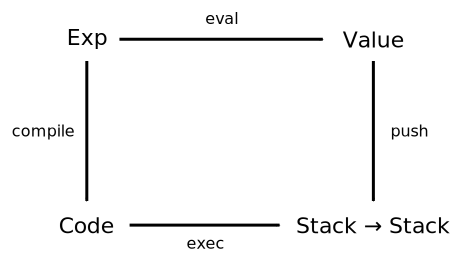
\includegraphics[width=0.75\textwidth]{correctness.pdf}
            \end{center}
        \end{frame}

        \begin{frame}
            %% João Pizani wants to present this :)
            \frametitle{Reference paper}
            \begin{itemize}
                \item "A type-correct, stack-safe, provably correct expression compiler in Epigram"
                    \begin{itemize}
                        \item James McKinna, Joel Wright
                    \end{itemize}

                \item Basic ideas and proofs, which we extended\ldots
            \end{itemize}
        \end{frame}
    

    \subsection{Sharing}
        \begin{frame}[fragile]
            %% João Pizani wants to present this :)
            \frametitle{Extending the source language}

            \begin{itemize}
                \item More "realistic" languages have sharing constructs
                \item We wanted the "simplest possible" extension with sharing behaviour.
                \item \textbf{Chosen extension: if\_then\_else $+$ sequencing}
                    \begin{verbatim}
if c then t else e >> common-suffix
                    \end{verbatim}
            \end{itemize}
            %% Wout draws "diamond" on the board

            \begin{itemize}
                \item The "naïve" compile function will duplicate the suffix
                \item Having Bytecode defined as graph (structured graph) instead of tree
                    would solve this problem
                    \begin{itemize}
                        \item But proofs would be more complex
                    \end{itemize}
            \end{itemize}
\end{frame}


    \subsection{Goals}
        \begin{frame}
            %% Wout presents this? :)
            \frametitle{What we ideally want}

            \begin{itemize}
                \item Have a "smart" graph-based compiler, generating code which uses sharing
                \item Write the correctness proof only for the "dumb" compiler,
                    have correctness \textbf{derived} for the smart version.
              \end{itemize}
        \end{frame}

        \begin{frame}
            %% Wout presents this? :)
            \frametitle{Reference paper}

            \begin{itemize}
                \item "Proving Correctness of Compilers using Structured Graphs"
                    \begin{itemize}
                        \item Patrick Bahr (visiting researcher)
                    \end{itemize}
            \end{itemize}
        \end{frame}

        \begin{frame}
            %% Wout presents this? :)
            \frametitle{Our project's goals}

            \begin{itemize}
                \item Integrating the best of both ``reference'' papers

                \item Our contributions:
                \begin{itemize}
                    \item (Simplest possible) language extension showing sharing behaviour.

                    \item Proof of correctness for the \textbf{stack-safe} ``naïve'' compiler
                        \begin{itemize}
                            \item The one that just duplicates code.
                        \end{itemize}

                    \item A way to to lift this \textbf{stack-safe} "naïve" correctness proof
                        \begin{itemize}
                            \item Into a proof concerning the more \textbf{efficient} compiler.
                        \end{itemize}
                \end{itemize}
            \end{itemize}
        \end{frame}

    \section{Implementation (code)}

    \subsection{Basic correctness}

        \begin{frame}[fragile]
            %% João Pizani wants to present this :)
            \frametitle{Source}

            Source types:
            \ExecuteMetaData[agda/tex/Source.tex]{tys}

            Source terms (snippet):
            \ExecuteMetaData[agda/tex/Source.tex]{src}

            Denotational semantics (snippet):
            \ExecuteMetaData[agda/tex/Source.tex]{eval}
\end{frame}

        \begin{frame}[fragile]
            \frametitle{Bytecode}
            %% João Pizani wants to present this :)

            Typed stack:
            \ExecuteMetaData[agda/tex/Bytecode.tex]{stacktype}
            \ExecuteMetaData[agda/tex/Bytecode.tex]{stack}

            Typed bytecode (snippet):
            \ExecuteMetaData[agda/tex/Bytecode.tex]{bytecode}
\end{frame}

        \begin{frame}[fragile]
            \frametitle{Compiler correctness}
            %% João Pizani wants to present this :)
            \ExecuteMetaData[agda/tex/Bytecode.tex]{compile}
            \begin{verbatim}
correct : {t : Tyₛ} {z : Sizeₛ} (e : Src t z)
        → exec (compile e) ≡ ⟦ e ⟧
            \end{verbatim}
\end{frame}


    \subsection{Lifting to sharing setting}
        \begin{frame}[fragile]
            \frametitle{Tree fixpoints}
            %% Wout presents this? :)
            Fixed Point for standard Functors
            \ExecuteMetaData[agda/tex/Bytecode.tex]{Tree}
            
            Fixed Point for indexed Functors
            \ExecuteMetaData[agda/tex/Bytecode.tex]{HTree}
\end{frame}

        \begin{frame}[fragile]
            \frametitle{Bytecode Tree Representation}
            %% Wout presents this? :)
            \ExecuteMetaData[agda/tex/Bytecode.tex]{bytecode}
            \ExecuteMetaData[agda/tex/Bytecode.tex]{bytecodeF}
            `Bytecode` is isomorphic to `HTree BytecodeF`:
            We have: `fromGraph . toGraph == id`
            And:     `toGraph . fromGraph == id`
\end{frame}
                
        \begin{frame}[fragile]
            \frametitle{Correctness on Trees}
            %% Wout presents this? :)
            \ExecuteMetaData[agda/tex/Bytecode.tex]{compileT}
            \ExecuteMetaData[agda/tex/Bytecode.tex]{execT}
            \begin{verbatim}
correctT : ∀ {t z s'} → (e : Src t z) 
         → execT (compileT e) ≡ ⟦ e ⟧
            \end{verbatim}
            The proof for `correctT` can be trivially lifted from `correct`,
            because `Bytecode` is structurally the same as `HTree BytecodeF`
\end{frame}

        \begin{frame}[fragile]
            \frametitle{Graphs}
            %% Wout presents this? :)
            % Sample code from page 9, showing let/var
            %
            \begin{verbatim}
data HGraph .. : ... -> Set where ...
            \end{verbatim}
            
            `HGraph` is like `HTree`, but with additional constructors to represent shared subtrees
            
            `Bytecode` is not exactly isomorphic to `HGraph BytecodeF`:
            We have: `fromGraph . toGraph == id`
            But:     `toGraph . fromGraph /= id`
            
            HGraph -> Bytecode -> HGraph loses sharing
\end{frame}
         
         \begin{frame}[fragile]
            \frametitle{Bytecode Graph Representation}
            %% Wout presents this? :)
            \ExecuteMetaData[agda/tex/Bytecode.tex]{compileG}
            \ExecuteMetaData[agda/tex/Bytecode.tex]{execG}
            \begin{verbatim}
correctG : ∀ {t z} → (e : Src t z) 
         → execG (compileG e) ≡ ⟦ e ⟧
            \end{verbatim}
            
            Using machinery, we get this proof automatically from `correctT`
\end{frame}


    \section{Equivalence of Graph and Tree compilers}

    \subsection{BytecodeF}


    \subsection{HTree and HGraph}


    \subsection{Equivalence Theorems}




    \begin{frame}[plain]
        \begin{center}
            \par{\Huge{Thank you!}}
            \vspace{2.0cm}
            \par{\Huge{Questions?}}
        \end{center}
    \end{frame}
\end{document}
